\chapter{Deep Learning Background}
TODO add intro

\section{Convolutional Neural Networks}
Convolutional Neural Networks (CNNs) are a Machine Learning model architecture which uses a filter, or kernel, convolved over the input to extract features relevant to the given kernel from a small area of the input.
Multiple kernels are used at each layer of the model to extract multiple features, known as feature maps, from a given input image.
The CNN architecture is often paired with a downsampling layer to reduce the number of parameters in the model and prevent the model from growing too deep and becoming difficult to train due to vanishing gradients.
An activation function is applied to the output feature map from each convolutional layer to add non-linearities to the model. 

\subsection{Convolutional Layers}
Each convolutional layer is made up of a number of learnable kernels which are applied to the entire input image by sliding the kernels across the width and height of the image taking the dot product of the kernel and the current receptive field of the kernel for all channels of the input image, as demonstrated in Figure \ref{fig:Conv_Layer}.
Each kernel is able to capture spatially relevant information about the current receptive field and pass this to the subsequent layers of the model.
During training these kernels are optimised to capture the most useful information for the task at hand.
The number of kernels used at each layer determines the number of feature maps produced, each of which are stacked as channels.
As each kernel is applied to the whole input image, the same learned parameters for each kernel are applied to the whole image, with each kernel extracting specific information.

\begin{figure}[h]
    \centering
        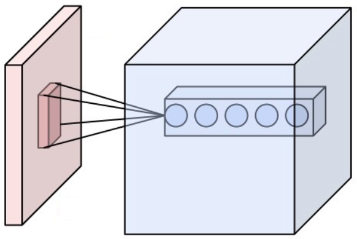
\includegraphics[width=0.5\textwidth]{figures/dl/conv_layer.png}
    \caption{Convolutional Layer}\label{fig:Conv_Layer}
\end{figure}

\subsection{Layer Output Sizes}
An issue with convolutional layers is that the output image is slightly smaller than the input image as the kernel cannot be applied over the edge of the image.
For a given kernel size, the output image size can be calculated with equation (\ref{eq:conv_output}), where $H_{in}$ and $H_{out}$ represent the input and output sizes along one dimension, $k$ represents the size of the kernel along that dimension, $p$ is the padding applied to the input image and $s$ is the stride at which the kernel is applied to the image.

\begin{equation} \label{eq:conv_output}
    H_{out} = \frac{H_{in} + 2p - k}{s} + 1
\end{equation}

Padding can be applied to the image to increase the size of the input such that the output image is of the same size.
Commonly zero padding is applied, such that the image is padded with zeros around its border.

\subsubsection{Reducing Layer Output Size}
In order to prevent the models from becoming too deep and to limit the number of trainable parameters in models, it is desirable to reduce the output feature map size.
To achieve this, pooling layers are commonly used, commonly either Max Pooling or Average Pooling.

Pooling layers apply a kernel over feature maps in a similar way to a convolutional layer, but apply a fixed function to the inputs rather than using learned parameters.
A Max Pooling layer will output the maximum value from each position, and discard the remaining values.
An Average Pooling layer will take the mean average of the values at each position.

An alternate method of reducing the size of the output feature maps is by increasing the stride of the convolutional layers, such that the kernel isn't applied at every position, but may skip positions.
Provided that the kernel size is larger than the stride of the convolutions, the whole feature map will still be covered.
One possible advantage of this is that the kernel values are learnt such that the model will be able to extract the most useful information given that the stride is not one for the layer.
By using a layer which learns given the use of strided convolutions, allows the model to learn to downsample feature maps in the manner which retains the most useful information.

\section{Activation Functions}
In order to add non-linearities to the model, activation functions are applied after each layer of models.
This non-linearity enables complex high order functions to be approximated by the network.
There exist many activation functions, but this section shall focus on those which have been used in the models proposed in the \textcolor{red}{\textbf{(TODO add link to methods section)}} section.
Activation functions are often selected based on the range of their output values, but in cases where this is unimportant it is common to use the Rectified Linear Unit (ReLU) function as it provides strong gradients, which aids in the prevention of vanishing gradients in deep network models, \cite{Goodfellow-et-al-2016}.

\begin{figure}[h]
    \centering
    \begin{subfigure}[b]{0.49\textwidth}
        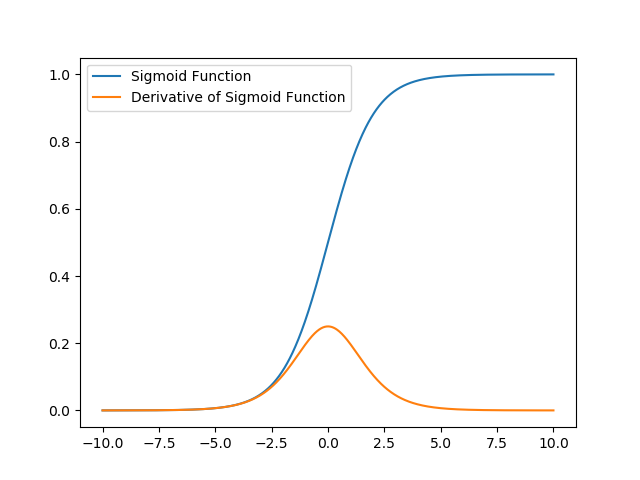
\includegraphics[width=\textwidth]{figures/dl/sigmoid.png}
        \subcaption{Sigmoid Function}\label{fig:Sigmoid}
    \end{subfigure}
    \begin{subfigure}[b]{0.49\textwidth}
        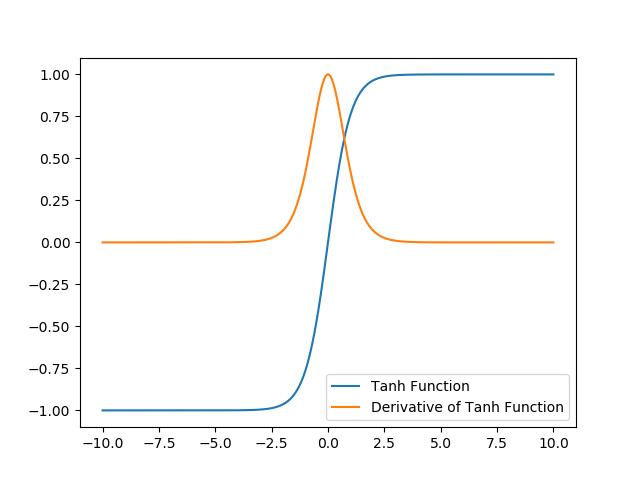
\includegraphics[width=\textwidth]{figures/dl/tanh.png}
        \subcaption{Tanh Function}\label{fig:Tanh}
    \end{subfigure}
    \begin{subfigure}[b]{0.49\textwidth}
        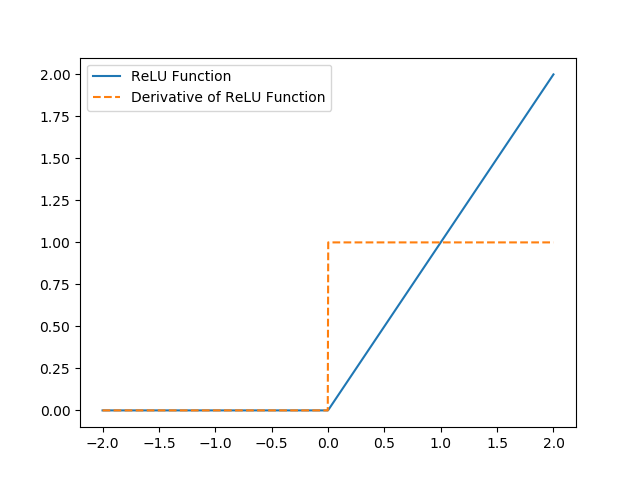
\includegraphics[width=\textwidth]{figures/dl/relu.png}
        \subcaption{ReLU Function}\label{fig:ReLU}
    \end{subfigure}
    \begin{subfigure}[b]{0.49\textwidth}
        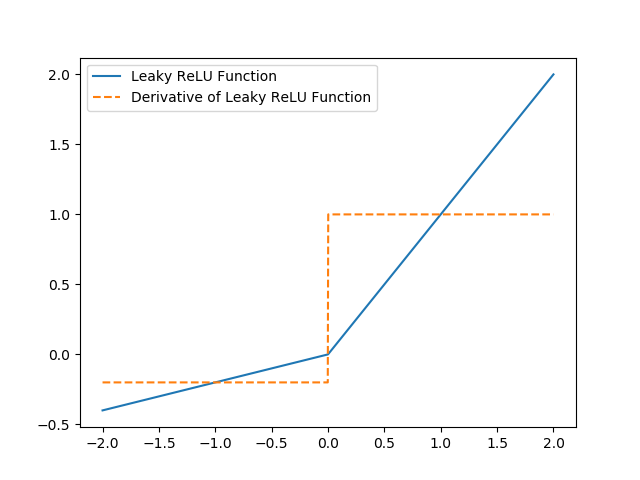
\includegraphics[width=\textwidth]{figures/dl/lrelu.png}
        \subcaption{LeakyReLU Function}\label{fig:LeakyReLU}
    \end{subfigure}
    \caption{Activation Functions}\label{fig:activations}
\end{figure}

\subsection{Sigmoid}
The Sigmoid function, expressed by equation (\ref{eq:sigmoid}) and shown in Figure \ref{fig:Sigmoid} is a logistic function which maps all real values to values within the range of 0 and 1.
A potential issue with the Sigmoid function is that the gradients at all points on the curve are small, with a maximum gradient of just 0.25 where $x = 0$.

\begin{equation}\label{eq:sigmoid}
    \sigma(x) = \frac{1}{1 + e^{-x}}
\end{equation}

\subsection{Tanh}
The Tanh function, expressed by equation (\ref{eq:tanh}) and shown in Figure \ref{fig:Tanh} is related to the Sigmoid function by equation (\ref{eq:sig_tanh})
The Tanh function maps all real values to the range of -1 and 1.
While the Tanh function has stronger gradients than the Sigmoid function, the gradients are still close to zero for most input values of $x$.

\begin{equation}\label{eq:tanh}
    \tanh(x) = \frac{e^x - e^{-x}}{e^x + e^{-x}}
\end{equation}

\begin{equation}\label{eq:sig_tanh}
    \tanh(x) = 2\sigma(2x) - 1
\end{equation}

\subsection{ReLU}
The ReLU function (Figure \ref{fig:ReLU}) is a non-linear function with strong gradient values for all input values of $x$ above zero.
Unlike the Sigmoid and Tanh function, the ReLU function is not differentiable everywhere due to the function not being continuous.
The gradient at the point where $x = 0$ is often treated as zero by library implementations to avoid this issue.

\begin{equation}\label{eq:relu}
    \text{ReLU}(x)=\begin{cases}
      x, & \text{if $x>0$}.\\
      0, & \text{otherwise}.
    \end{cases}
\end{equation}

While the ReLU function has a positive gradient where $x > 0$, the gradient is 0 where $x < 0$.
Another proposed activation function is the LeakyReLU function (Figure \ref{fig:LeakyReLU}) described by equation (\ref{eq:lrelu}) where $l$ is a selected parameter.
The LeakyReLU function multiplies the input value $x$ by some parameter $l$, where $l < 1$, such that $x$ is attenuated.

\begin{equation}\label{eq:lrelu}
    \text{LeakyReLU}(x)=\begin{cases}
      x, & \text{if $x>0$}.\\
      lx, & \text{otherwise}.
    \end{cases}
\end{equation}

\subsection{Softmax} \label{softmax}
The Softmax function is commonly used in classification problems in which a model aims to classify an input value $\bm{x}$ as one of $N$ labels.
The Softmax function, expressed by equation (\ref{eq:softmax}), converts the input $\bm{x}$ into a normalised probability distribution over the $N$ labels, the label with the highest likelihood is interpreted as the model's prediction. 
Such models are commonly trained with the Negative Log Likelihood loss function, by applying the log to the output of the softmax function.

\begin{equation}\label{eq:softmax}
    \text{Softmax}(x_i) = \frac{e^{x_i}}{\sum_j^N e^{x_j}}
\end{equation}

TODO add LogSoftmax...

TODO add NLL loss function

\section{Optimisation Algorithms}
With the aim of finding the model parameter values which minimise the loss function of the model, Gradient Descent algorithms are commonly used to find such parameters.
Given a loss function $L(x)$ which is to be minimised, where $x$ represents the model parameters, the value of $x$ is iteratively updated by calculating the gradient of $L(x)$ for the current parameters and updating the parameters as described by equation (\ref{eq:gradient_descent}).
$\epsilon$ is the learning rate for the algorithm which determines the step size made at each update.
Too large a step size and the update may overshoot the optimum value, too small a step size may result in a model which takes an impractical length of time to train. 
It's is often useful in practice to begin with a learning rate which is able to make large steps, then to reduce the learning rate $\epsilon$ as the model trains.

\textcolor{red}{\textbf{(TODO add graphical examples)}}

\begin{equation}\label{eq:gradient_descent}
   x^\prime = x - \epsilon \nabla_x L(x)
\end{equation}

\subsection{Stochastic Gradient Descent}
Stochastic Gradient Descent (SGD) takes a minibatch of $m$ samples from a data generating independent and identically distributed (i.i.d) distribution, and calculates the average gradient with which the update rule described by equation (\ref{eq:SGD}) is applied.
The use of minibatches results in an approximation of the true gradient as the whole dataset is not evaluated before making an update, just a small subset of the dataset.
This can have the affect of adding regularisation to the learning procedure, particularly with smaller batch sizes \cite{Goodfellow-et-al-2016}.
The SGD update rule for a loss function $L(.)$ and model $f(\bm{x}_i; \bm{\theta})$ can be defined by equation (\ref{eq:SGD}):

\begin{equation*}
    \bm{g} = \frac{1}{m} \nabla_\theta \sum_i^m L(f(\bm{x}_i; \bm{\theta}), y_i)
\end{equation*}

\begin{equation}\label{eq:SGD}
    \bm{\theta}^\prime = \bm{\theta} - \epsilon \bm{g}
\end{equation}

where $\bm{g}$ represents the approximation of the gradient, $\bm{\theta}$ represents model parameters and $\bm{x}_i$ represents $m$ samples making up the minibatch $\{\bm{x}_1, \dots, \bm{x}_m\}$ and corresponding target values $\bm{y}_i$.

\subsection{Momentum}
In order to the accelerate the training of models and find the global minimum faster, momentum is often used with optimisation algorithms.
In addition to the gradient term, a velocity term is also calculated as an accumulation of decaying moving average values from the previous gradient approximation \cite{Goodfellow-et-al-2016}.
The result of this is that the optimisation will continue to move in the direction in which it has been moving, aiding in the prevention of the model becoming stuck in local minimum.
Figure \ref{fig:Momentum} demonstrates how momentum may accelerate the optimisation process.
Here the black arrows represent the gradient evaluated at each point, while the red line shows the path taken with momentum.

\begin{figure}[h]
    \centering
        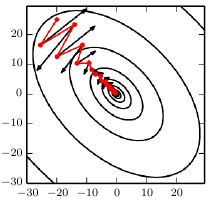
\includegraphics[width=0.3\textwidth]{figures/dl/momentum.png}
    \caption{SGD with Momentum \cite{Goodfellow-et-al-2016}}\label{fig:Momentum}
\end{figure}

\subsubsection{Adaptive Learning Algorithms}
Such algorithms as RMSprop and Adam exist which are built upon the principles of the SGD algorithm with the addition of momentum but adapt their learning rates or momentum values based on a history of previous gradient values.
These aid in finding the global minimum for the loss function at hand.

TODO More details on RMSprop